
\documentclass[PICOReport.tex]{subfiles}

\begin{document}

%Enumerate the various signals in polarization. Use the frequency band + signals figure. The challenge is to dig out the faintest of all signals, the one due to $r$. This sets the tone for the entire 'signal decomposition' or 'component separation'.  Removing the galactic signal to unmask $r \lesssim 0.001$ is a challenge for all future experiments searching for $r$ at that level, and is a strong advantage of a space platform. The physics of galactic signals suggests complexities in their combined emission properties; the level of this complexity is not known. } 

Diffuse Milky Way emissions dominate the sky's polarized intensity on the largest angular scales; see Figures~\ref{fig:clbb} and ~\ref{fig:pico-channels-and-fg}. Polarized radiation arises primarily from the synchrotron emission of energetic electrons spiralling in the magnetic field of our own Galaxy, and from thermal
emission from elongated interstellar dust grains. Although the levels of these foreground emissions decrease with decreasing angular scales, they can still be considerably brighter 
than the \ac{IGW} peak around $\ell=80$ when averaging over 60\% of the sky. 
In fact, even in the cleanest, smaller patches of the sky, far from the galactic plane and thus relatively low in galactic emissions, their levels are expected to be substantial relative to the \ac{IGW} for $r \lesssim 0.01$, and dominate it for $r \lesssim0.001$. Separating the cosmological and Galactic emissions signals, also called foreground separation, together with control of systematic uncertainties are {\it the} challenges facing any next decade experiment attempting to reach these levels of constraints on $r$.

\begin{figure}[ht]
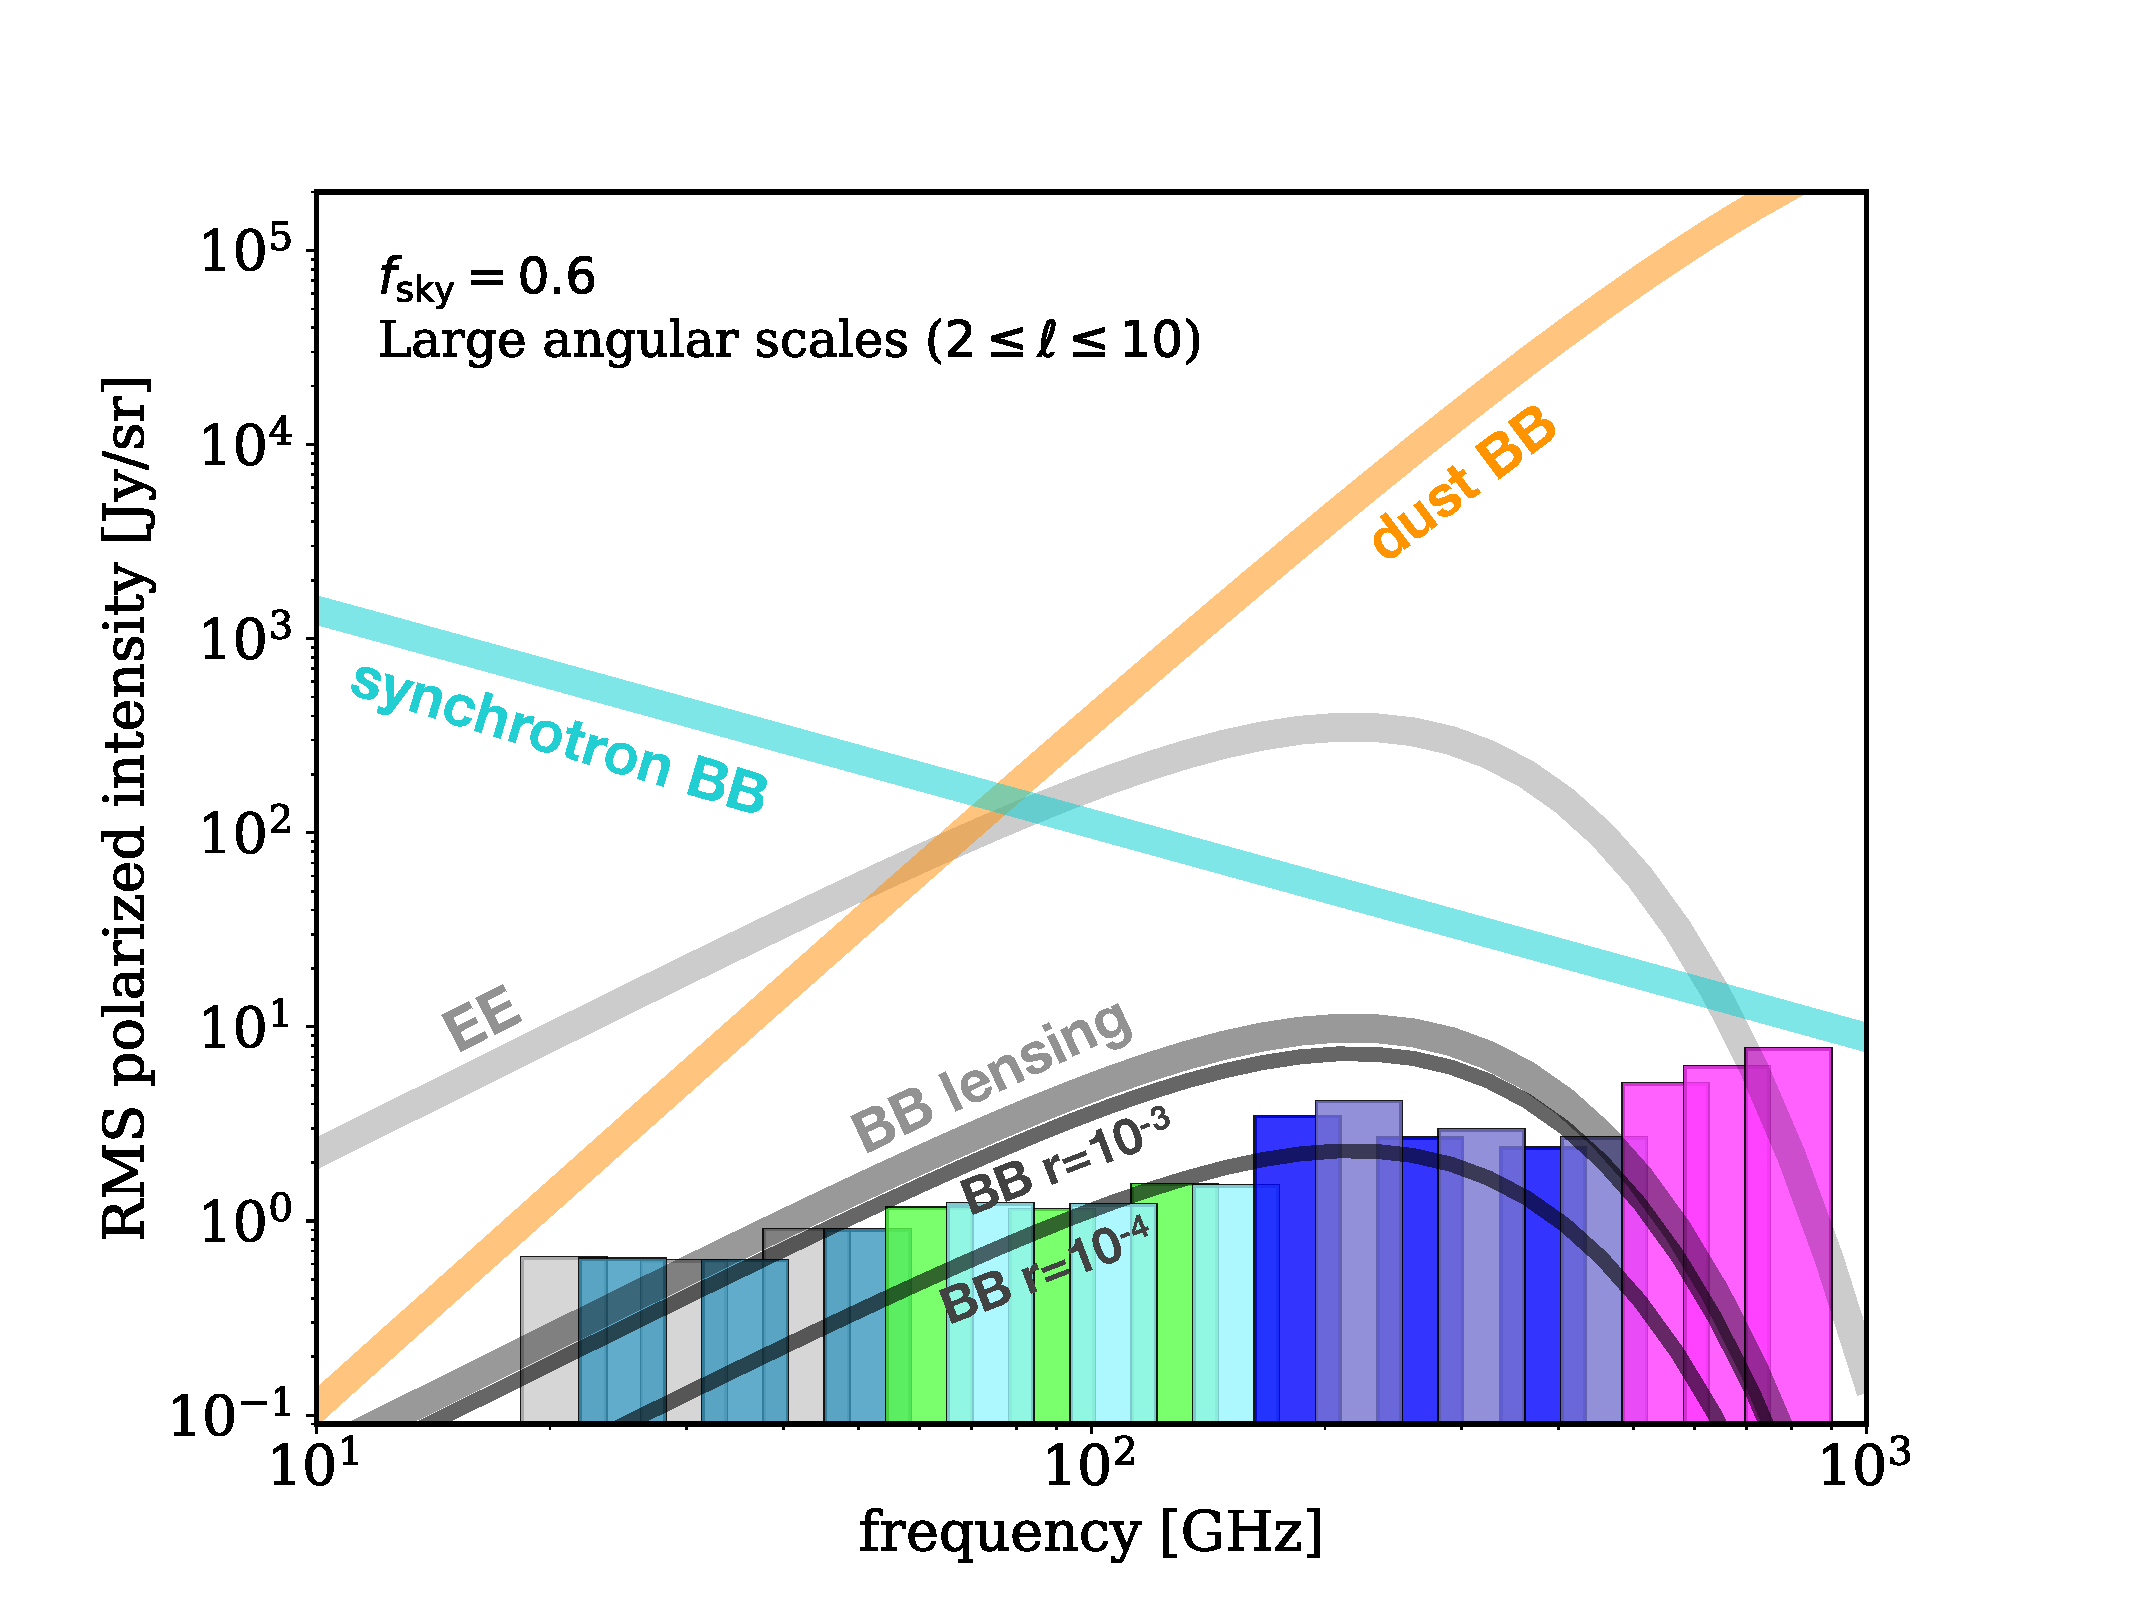
\includegraphics[width=0.49\textwidth]{images/sensitivity_vs_frequency_Jun29th_2018_large.pdf}
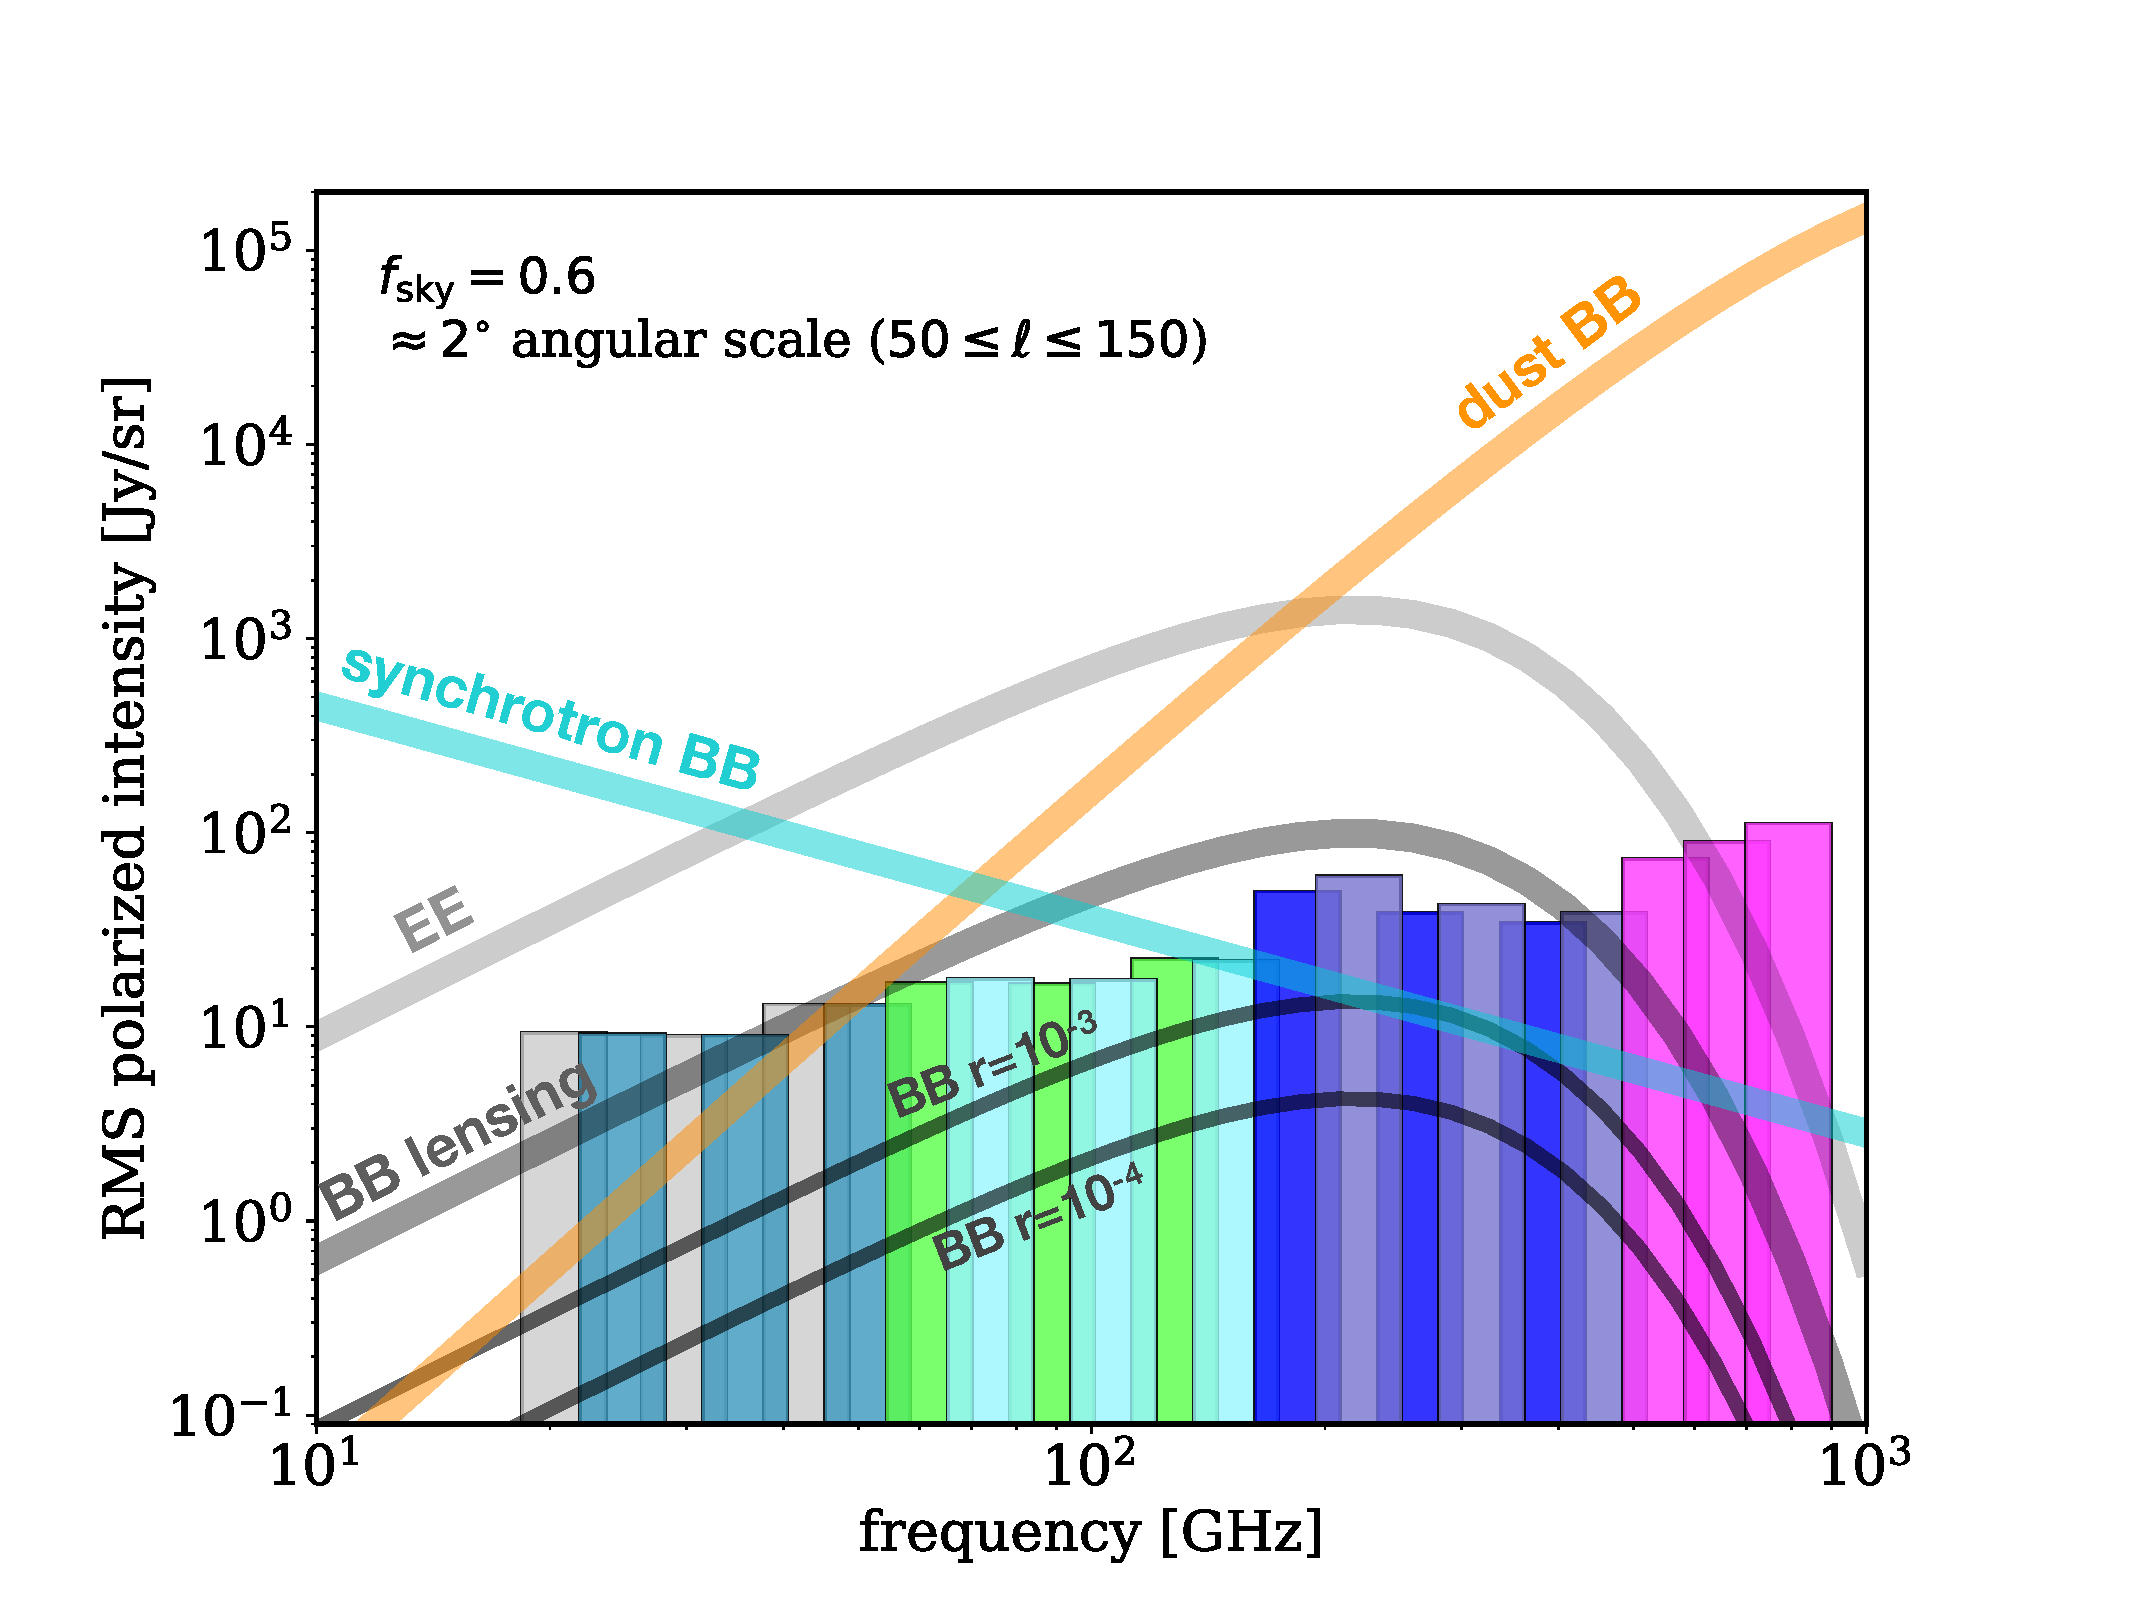
\includegraphics[width=0.49\textwidth]{images/sensitivity_vs_frequency_Jun29th_2018_2deg.pdf}
\vspace{-0.1in}
\caption{Polarization $BB$ spectra of Galactic synchrotron and dust, compared to CMB polarization $EE$ and $BB$ spectra of different origins for two values of $r$ and for two ranges of angular scales: large $\ell \leq 10$ corresponding to the reionization peak (left panel), and intermediate $50 \leq \ell \leq 150$ corresponding to the recombination peak (right panel). The location and sensitivity of the 21 PICO frequency channels is shown as vertical bands. (The color scheme is explained in Section~3.2.) }
\label{fig:pico-channels-and-fg}
\end{figure}

The foreground separation challenge would be easily surmountable if the Galactic emissions were %already 
precisely characterized, or were known to have simple, fittable spectral emission laws. But neither is true. To first order, the spectrum of Galactic synchrotron emission, arising from free electrons spiraling around Galactic magnetic fields, can be modeled as a power law $I_{\rm sync} \propto \nu^{\alpha},$ with $\alpha \simeq -1$ (in brightness units). The spectrum of Galactic dust emission, arising from emission by Galactic dust grains, can be modeled as $I_{\rm dust} \propto \nu^{\beta} B_\nu(T_{\rm dust}),$ where $\beta \simeq 1.6$, $T_{\rm dust} \simeq 19$\,K, and $B_\nu(T)$ is the Planck function; this is referred to as `modified black body emission'. If those models were exact, then in principle, an experiment that had 6 frequency bands could determine the three emission parameters as well as the three amplitudes corresponding to that of dust, synchrotron, and the CMB. However, recent observations have shown that neither emission law is universal, that spectral parameters vary with the region of sky \cite{SPASS_2018_variation,fuskeland2014_wmap_variation,planck_2013_xi}, and thus that the analytic forms and parameter values given above are valid only as averages across the sky. Also, while both emission laws are well-motivated phenomenological descriptions, the fundamental physics of emissions from grains of different materials, sizes and temperatures, and of electrons spiraling around magnetic fields implies that these laws are not expected to be exact, nor universal. 

Additional polarized foregrounds may exist.  `Anomalous microwave emission' (AME) is observed at mm wavelengths, spatially correlated with thermal dust emission but with intensity peaked at frequencies near 30 GHz.  While not
known to be polarized, even a small (0.1\%) fractional polarization would be appreciable for $\sigma(r) \lesssim 0.001$.  Astrophysical emission from CO lines at mm wavelengths, and even small polarization of radio and infrared sources at shorter wavelengths could also complicate polarized signal separation~\citep{trombetti2018_fracpol, puglisi2018_polsource}.

PICO will dramatically improve sensitivity to inflationary B-modes. The improved sensitivity requires concurrent improvements in foreground separation.  Simple foreground models, suitable for the current generation of CMB measurements, will fail at the higher PICO sensitivity.  For example, the Planck modified blackbody model assumes that interstellar dust emits at a single temperature, which is clearly an approximation to the more complicated emission along lines of sight spanning hundreds of pc. Several publications have demonstrated that fitting complicated temperature profiles using a simple one- or two-temperature model will bias the fitted CMB signal at levels $\delta r \lesssim 10^{-3}$, large compared to the PICO goal~\citep{fantaye2011,armitage-caplan2012,kogut_fixsen2016,remazeilles/etal:2016,stompor2016}.


%Faced with these uncertainties, but also with the opportunity provided by a platform that can host a broad range of frequencies -- ground-based experiments are limited to several atmospheric windows and to frequencies of less than 300~GHz -- PICO is designed with 21 frequency bands between 21 and 800 GHz; see Figure~\ref{fig:pico-channels-and-fg} and Table 3.2. This is the broadest frequency lever arm proposed by any imaging instrument to characterize and enable separation of Galactic emissions. 

Foreground uncertainties, and the level of fidelity required in their characterization, also compel a transition in the way we assess and forecast the performance of a future experiment. We can no longer impose specific models upon the data; rather, the data collected should provide information to constrain Galactic emissions with sufficient accuracy.  Two broad techniques are available.  Parametric models use the frequency dependence of the data in each line of sight to determine the effective frequency dependence of foreground emission.  Since the CMB spectrum is well determined, measurements with sufficiently broad frequency coverage can distinguish foreground emission from the CMB component by their different spectral dependences.  Non-parametric techniques, in contrast, rely on the fact that CMB emission is uncorrelated with the foregrounds and use both spatial and frequency correlations within a spatial/frequency data cube to separate CMB from foreground components.  Simulated data assess the efficacy of both techniques as a function of increasing complexity for the assumed foreground emission.

To investigate the capacity of PICO to address this foreground separation problem, we use the approach that has become the `gold standard' in the community. In this approach we simulate sky maps that are constrained by available data, but otherwise have a mixtures of foreground properties. We  `observe' these maps just like a realistic experiment will do, and then apply foreground separation techniques to separate the Galactic and CMB emissions. We also provide forecasts using other techniques that use analytic calculations to estimate the efficacy of foreground separation, or others in which the simulated sky map is assumed to have specific Galactic emission models, which are then being fitted. 
\begin{figure}[t]
\begin{center}
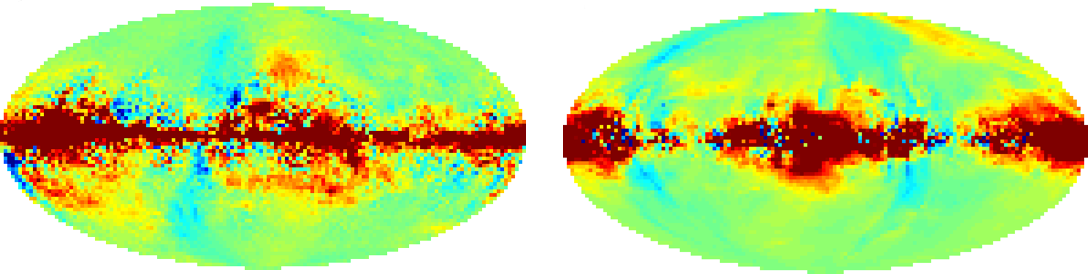
\includegraphics[width=.8\textwidth]{images/pysm_foregrounds_155GHz.png}
\vspace{-0.1in}
\caption{Foregrounds models at 155~GHz from PySM (left)~\citep{thorne2018_pysm} and Galactic MHD simulations (right). }
\label{fig:pysm_foregrounds}
\end{center}
\vspace{-0.2in}
\end{figure}



%Foreground uncertainties, and the level of fidelity required in their characterization, also compel a transition in the way we assess and forecast the performance of a future experiment. We can no longer impose specific models upon the data. Rather, the data collected should provide information to constrain Galactic emissions with sufficient accuracy. For PICO we use the approach that has become the `gold standard' in the community. In this approach we simulate sky maps that are constrained by available data, but otherwise have a mixtures of foreground properties, observe these maps just like a realistic experiment will do, and then apply foreground separation techniques to separate the Galactic and CMB emissions. We also provide forecasts using other techniques that use analytic calculations to estimate the efficacy of foreground separation, or others in which the simulated sky map is assumed to have specific Galactic emission models, which are then being fitted. 

%\comor{now need to connect to the next paragraphs} As we show below, the PICO broad frequency coverage, coupled with high sensitivity enables studying the sky using the PICO data themselves rather than assuming what the sky is, and fitting our models to these assumptions. 

%%%%%%%%%%%%%%%%%%%%%%%%%%%%%%%%%%%
\subsubsection{PICO Foreground Separation Methodology}
%%%%%%%%%%%%%%%%%%%%%%%%%%%%%%%%%%%

%\noindent{\bf Sky Maps} \hspace{0.1in} 
For assessing the efficacy of foreground separation with PICO we used 8 different full sky models. All models were broadly consistent with available data and uncertainties from WMAP and \planck . The range of models included one test case that had a very simple realization of foregrounds, and others with varying degree of complexity including spectral parameters varying spatially and along the line of sight, anomalous microwave emission up to 2\% polarized, dust polarization that rotates slightly as a function of frequency because of projection effects, or dust spectral energy distribution that departs from a simple modified blackbody. All foreground maps were generated at native resolution of 6.8 arcmin pixels~\citep{healpix}. They were generated using PySM and/or PSM codes~\citep{thorne2018_pysm,delabrouille/etal:2013}.   Distinctly different realizations of the sky are allowed by current data, as demonstrated by Figure~\ref{fig:pysm_foregrounds}. 
%\comor{ Karl, More details of the models are available at~\citet{foregroundappendix}.}


For each of the 8 models we added CMB signals in both intensity and polarization matching a $\Lambda$CDM universe. The $BB$-lensing signal matched the level of 85\% delensing forecasted for PICO. Each of these sky models had 100 different realization of the PICO CBE noise levels; 50 realizations had no \ac{IGW} signal and 50 others had a level of $r=0.003$. 
%\vspace{0.1in}
%\noindent{\bf Foreground Separation} \hspace{0.1in} 
The sky models were analyzed with a variety of techniques which were based on the two broad categories described above. 

%: correlation methods, which exploit the fact that foreground emission is strongly correlated from frequency to frequency, but uncorrelated with the CMB, and parametric methods, which model the sky emission using specific (parametric) emission laws, and use spectral fits in independent pixels or sky regions to infer the amplitude and spectral parameters of each of the components in the sky. Correlation methods include SEVEM, and variants of the \ac{ILC} algorithm, such as the needlet-space \ac{ILC} (NILC) and a version generalised to multidmensional components (GNILC). Parametric methods include the Commander algorithm.
Analytic forecasts were based on a Fisher information matrix approach~\citep{errard_feeney_2016} and included foreground separation
%run using the CMB4cast Fisher matrix code (http://portal.nersc.gov/project/mp107/index.html, Errard & Feeney et 
%access to $TT$, $E, B and d information, with the deflection estimated using the iterative EB estimator. The code 
%Planck-2015-level synchrotron and dust foregrounds, forecasting the experiment's ability to clean these foregrounds 
using a parametric maximum-likelihood approach, assuming the foreground spectral indices are constant on patches of size ~15 degrees across. 
%This is all probably a little out-of-date, being based on the Planck 2015 results and cosmology, but it doesn't seem to give a significantly different answer to Raphael's code (and I can rerun with a different tau if you'd like).

%\comor{say something about the fisher methods, Raphael and Stephen}

%\vspace{0.1in}
%\noindent{\bf Acknowledged Limitations} \hspace{0.1in} The level of effort supported 

%%%%%%%%%%%%%%%%%%%%%%%%%%%%%%%%%%%
\subsubsection{Results and Discussion}
%%%%%%%%%%%%%%%%%%%%%%%%%%%%%%%%%%%

There is evidence that at levels of $r \simeq 0.001$ the combination of PICO's sensitivity and broad frequency coverage are efficacious in foreground removal. Figure~\ref{fig:nilc} shows a result from the gold standard process described above for one of the sky models and with an input \ac{IGW} of $r=0.003$. Residual foregrounds are below the cosmological signal over the important low $\ell$ range, where foregrounds are strongest. The residual spectra would likely be lower when analysis is carried out on only 50 or 40\% of the sky, rather than the 60\% used here. 

\begin{figure}
\hspace{-0.1in}
\parbox{3.0in}{\centerline {
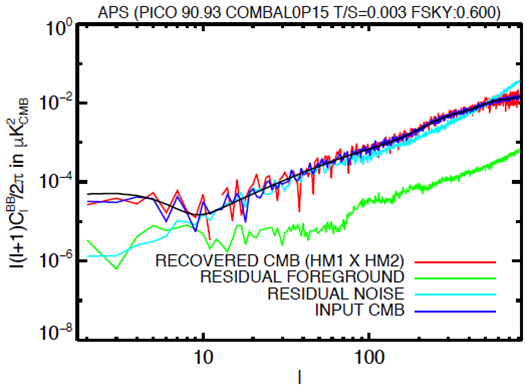
\includegraphics[width=3.0in]{images/soumen_NILC_foregrounds_93.png}}}
\hspace{0.25in}
\parbox{3.0in}{
\caption{The power spectrum of residual $BB$ foregrounds (green) has lower level than both the input CMB (blue) and the recovered CMB (red) which match well each other and the underlying cosmological model (black) after foreground separation with the NILC algorithm. This exercise assumed use of 60\% of the sky.   
\label{fig:nilc}}}
\vspace{-0.1in}
\end{figure}

Our results validate the need for a broad frequency coverage with a strong lever arm on Galactic emissions outside of the primary CMB bands. Figure~\ref{fig:commander} shows that removing several of PICO's frequency bands, particularly those that monitor dust and synchrotron at high and low frequencies, respectively, significantly biases the extracted $BB$ power spectrum, particularly at the lowest $\ell$ values. 


There is other evidence that PICO could reach its stated target of $\sigma(r) = 0.0001$. Map-based simulations that were carried out for the forthcoming CMB-S4 experiment have shown that it can reach levels of $\sigma(r) = 0.0005$ in small, 3\%-size, clean patches of the sky. The analysis only used frequencies up to 300~GHz. In principle, even smaller patches of 1-2\% size are sufficient, and preferable, for attaining as low $\sigma(r)$ as possible. The PICO noise level per sky pixel is similar to that of CMB-S4, but PICO will have {\it full} sky coverage and thus access to {\it all} the clean patches available. Data from \planck\ indicate that there are $\sim10$ %\comor{check!} 
patches as clean, or cleaner than those used for the CMB-S4 analysis, indicating that PICO's $\sigma{r}$ could be $\sim3$ times more stringent. This scaling is very conservative because it only assumes CMB-S4's much narrower breadth of frequency coverage and its 7 bands; % \comor{check}; 
it neglects PICOs much stronger rejection of foregrounds with 21 bands and up to 800~GHz.  We note that if there {\it is} a detection of the \ac{IGW} signal with $r=0.001$, PICO will make it with high significance in multiple independent patches of the sky. 

Results from the Fisher-based analytic calculations give $\sigma(r) = 9 \cdot 10^{-5}$, and indicate a very small foreground residual with an $r_{eff} = 9 \cdot 10^{-7}.$

While our results are encouraging, as they suggest that PICO's frequency coverage and sensitivity will be adequate for this level of $r$, more work should be invested to gain complete confidence. This work includes running numerous realizations of different sky models, and analyzing them with various techniques; optimizing sky masks; and using combination of techniques to handle large, intermediate, and small angular scale foregrounds differently. 
\begin{figure}
%\hspace{-0.1in}
%\parbox{4.5in}
{\centerline {
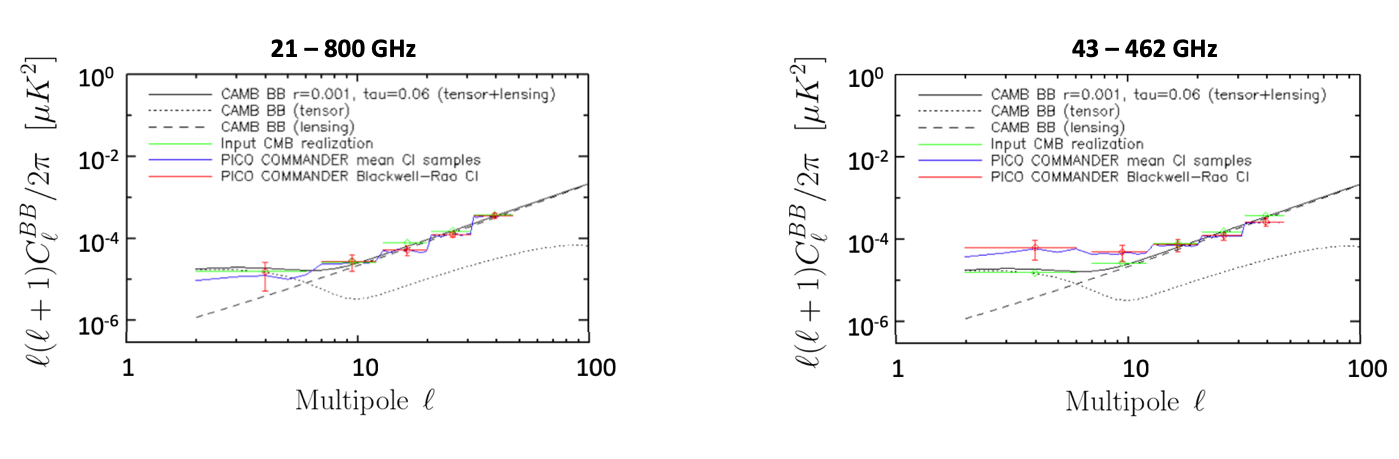
\includegraphics[width=4.5in]{images/commander_foregrounds_BB.png} }}
%\hspace{0.in}
%\parbox{2.0in}{
\caption{Foreground removal with all of PICO's 21 frequency bands (left panel) recovers the input CMB (green) without any bias (red) using the Commander algorithm on the \planck\ sky model (with 4~deg pixels, and 50\% sky fraction). Running the same algorithm on the same sky without several of the lowest and highest bands (right panel) produces an output spectrum (red) that is biased relative to the input (green) at low $\ell$ multipoles. The bias would be interpreted as higher value of $r$ relative to the model input (solid black) with $r=0.001$ (dots) and lensing (dash). 
\label{fig:commander}}
\vspace{-0.0in}
\end{figure}


%\begin{figure}
%\hspace{-0.1in}
%\parbox{4.5in}{\centerline {
%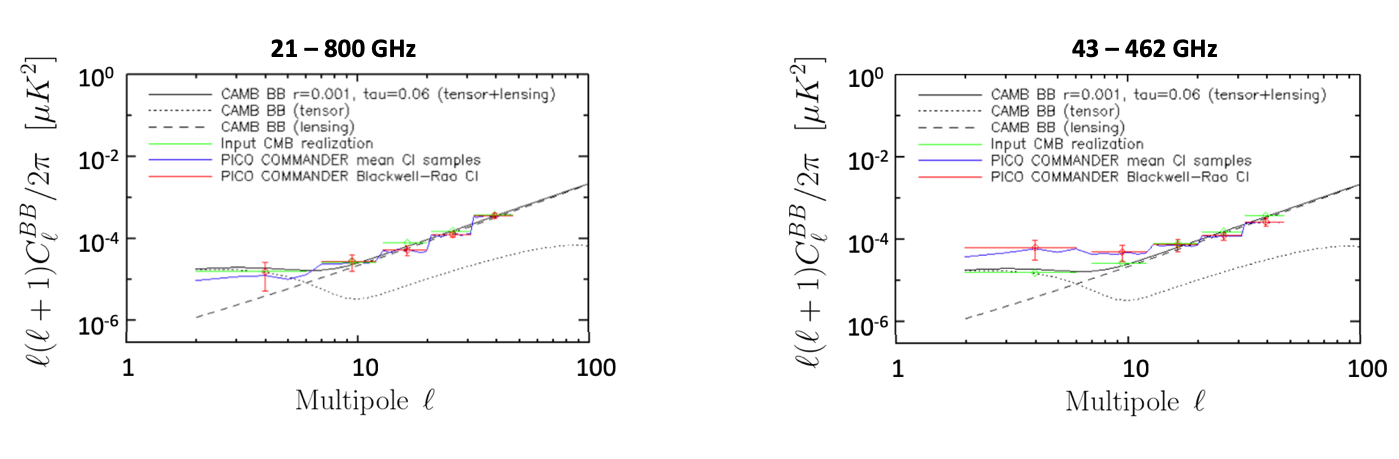
\includegraphics[width=4.5in]{images/commander_foregrounds_BB.png}}}
%\hspace{0.in}
%\parbox{2.0in}{
%\caption{Foreground removal with all of PICO's 21 frequency bands (left panel) recovers the input CMB (green) without any bias (red) using the Commander algorithm on the \planck\ sky model (with 4~deg pixels, \comor{and 60\%} sky fraction). Running the same algorithm on the same sky without the lowest and highest bands (right panel) produces an output spectrum (red) that is biased relative to the input (green) at low $\ell$ multipoles. The bias would be interpreted as higher value of $r$ relative to the model input (solid) with $r=0.001$ (dots) and lensing (dash). 
%\label{fig:commander}}}
%\vspace{-0.1in}
%\end{figure}


\end{document}

%\begin{figure}[!htb]
%\centering
%
\includegraphics[width=4cm]{images/example}
%\caption{example}
%\label{fig:im_3}
%\end{figure}

%The most important lesson arising from our exercise is that more work is required to ascertain that levels of $r \lesssim 0.001$ can be determined robustly on the largest angular scales, that is from the reionization peak.  Figure~\ref{fig:nilc} shows results from the NILC analysis. For several of the sky models the power spectra of the residual level of foregrounds -- that is the level of foregrounds remaining in the map after foreground separation -- is below the cosmological \ac{IGW} level with $r =0.003$. For a minority of the models, the residual is higher at $\ell \lesssim 20$. Results from GNILC, shown in Figure~\ref{fig:gnilc}, are similar. In all cases, the analyses are carried out using 60\% of the sky, the results shown are from one realization, and that no further optimization of the basic foreground separation technique has yet been applied. 

%More work is also required to understand the necessary span of frequencies required. Figure~\ref{fig:psm_mr} shows that removing several of PICO's frequency bands, in this case the three highest, significantly biases the extracted $BB$ power spectrum, particularly at the lowest $\ell$ values. This result should not be interpreted as conclusively demonstrating that a frequency span up to 800 GHz has been proven to be essential. At this point of time, different input sky models, coupled to different foreground separation techniques may yield different results. Rather, the conclusion is that further improvement in our modeling and analysis is required. 



%The baseline design of PICO has 21 channels observing the sky in the 20\,GHz to 800\,GHz frequency range (Fig.~\ref{fig:pico-channels-and-fg}). By analysing how the total emission varies across frequency bands, one can infer the detailed emission properties of the various emission components, form linear combinations of the observations that maximise the contribution of a component of interest while minimising contamination by the others and by instrumental noise, and understand the properties of the foregrounds to evaluate potential residuals in the CMB B-mode map. Various such techniques have been successfully used in previous CMB observations such as those of the Planck mission. Building on this existing expertise, we have carried out map based simulations within a ``data challenge'' framework to assess the capacity of PICO to measure the main signal of interest (CMB primordial B-modes). In this process one group prepares sets of simulated maps for different models of foreground emission of varying complexity from optimistic to pessimistic, which are placed in a shared area. These are then re-analyzed by multiple individuals and groups employing various different component separation algorithms.

